%! Author = Len Washington III
%! Date = 11/20/2023

% Preamble
\documentclass[27]{cs430lecture}

% Packages

% Document
\begin{document}

%<*Lecture-Activity-27>
\maketitle
\section{Shortest Path Problem}\label{sec:shortest-path-problem}
How to find the shortest route between two points on a map.
\subsection{Input}\label{subsec:shortest-path-input}
\begin{itemize}
	\item Directed graph $G=(V,E)$
	\item Weight function $w:E\rightarrow \mathbf{R}$
\end{itemize}

\subsection{Weight of path}\label{subsec:shortest-path-weight}
\begin{equation*}
\begin{aligned}
	p &= \langle v_{0}, v_{1}, \dots, v_{k} \rangle\\
	  &= \sum_{i=1}^{k} w(v_{i-1},v_{i})\\
	  &= \mbox{sum of edge weights on path }p.
\end{aligned}
\end{equation*}

\subsection{Shortest-path weight $u$ to $v$}\label{subsec:shortest-path-weight-u-to-v}
\[ \delta(u,v) = \left\{ \begin{array}{ll}
	\min\{ w(p): u\leadsto^{p} v & \mbox{if there exists a path }u\leadsto v, \}\\
	\infty & \mbox{otherwise.}
\end{array} \right. \]

Shortest path $u$ to $v$ is any path $p$ such that $w(p)=\delta(u,v)$.

Variants
\begin{itemize}
	\item Single-source: Find shortest paths from a given source vertex $s\in V$ to every vertex $v\in V$.
	\item Single-destination: Find shortest paths to a given destination vertex.
	\item Single-pair: Find shortest path from $u$ to $v$.
	No way known that's better in worst case than solving single-source.
	\item All-pairs: Find shortest path from $u$ to $v$ for all $u,v\in V$.
	We'll see algorithms for all-pairs in the \hyperref[sec:all-pairs-shortest-paths-problem]{next chapter}.
\end{itemize}

Negative-weight edges --
OK, as long as no negative-weight cycles are reachable from the source.
\begin{itemize}
	\item If we have a negative-weight cycle, just keep going around it, and get $w(s,v)=-\infty$ for all $v$ on the cycle.
	\item But OK if the negative-weight cycle is not reachable form the source.
	\item Some algorithms work only if there are no negative-weight edges in the graph.
\end{itemize}

\begin{enumerate}
    \item What would the brute force approach be to solve the shortest path problem, and what is its run time?
	\begin{answer}
		\begin{equation*}
		\begin{aligned}
			1 & \mbox{ Path of 1 edge}\\
			|V|-2 & \mbox{ Paths of 2 edges}\\
			(|V|-2)(|V|-3) & \mbox{ Paths of 3 edges}\\
			&\vdots\\
			|V|! & \mbox{ Paths of V edges}\\
		\end{aligned}
		\end{equation*}
	\end{answer}
	\item Prove \hyperref[dfn:optimal-substructure]{optimal substructure} for the shortest path problem.
	\begin{answer}
		Since shortest paths contain shortest subpaths (optimal solution to subproblem must in in optimal answer to problem.)
		$G\{V,E\}$, weight function on edge given source $v$, find shortest path to $u$
	\end{answer}
\end{enumerate}

Output of single-source shortest-path algorithm
For each vertex $v\in V$:
\begin{itemize}
	\item $d[v] = \delta(s,v)$,
	Initially, $d[v]=\infty$; reduces as algorithms progress.
	But always maintain $d[v]\gets \delta(s,v)$.
	Call $d[v]$ a shortest-path estimate.
	\item $\pi[v] = $ predecessor of $v$ on a shortest path from $s$.
	If no predecessor, $\pi[v]=NIL$, $\pi$ induces a tree--\emph{shortest-path tree}.
\end{itemize}

Initialization -- All the shortest-paths algorithms start with \Call{Init-Single-Source}{}.
\begin{algorithm}[H]
	\caption{Single Source Initialization}\label{alg:init-single-source}
	\begin{algorithmic}[1]
	\Function{Init-Single-Source}{$V$, $s$}
		\ForAll{$v\in V$}
			\State $d[v]\gets\infty$
			\State $\pi[v]\gets$ NIL
		\EndFor
		\State $d[s]\gets 0$
	\EndFunction
	\end{algorithmic}
\end{algorithm}

Relaxing an edge $(u,v)$ - Can we improve the shortest-path estimate (best seen so far)
from the source $s$ to $v$ be going through $u$ and taking edge $(u, v)$?

\begin{table}
    \centering
	\label{tab:relax}
	\begin{tabular}{|c|c|}
		\toprule
		\begin{minipage}[t]{0.45\textwidth}
			\begin{algorithm}[H]
				\caption{Relaxing an Edge}\label{alg:relax}
				\begin{algorithmic}[1]
				\Function{Relax}{$u$, $v$, $w$}
					\If{$d[v] > d[u] + w(u,v)$}
						\State $d[v]\gets d[u] + w(u,v)$
						\State $\pi[v]\gets u$
					\EndIf
				\EndFunction
				\end{algorithmic}
			\end{algorithm}
		\end{minipage} & \begin{minipage}[t]{0.55\textwidth}
			\begin{figure}[H]
				\centering
				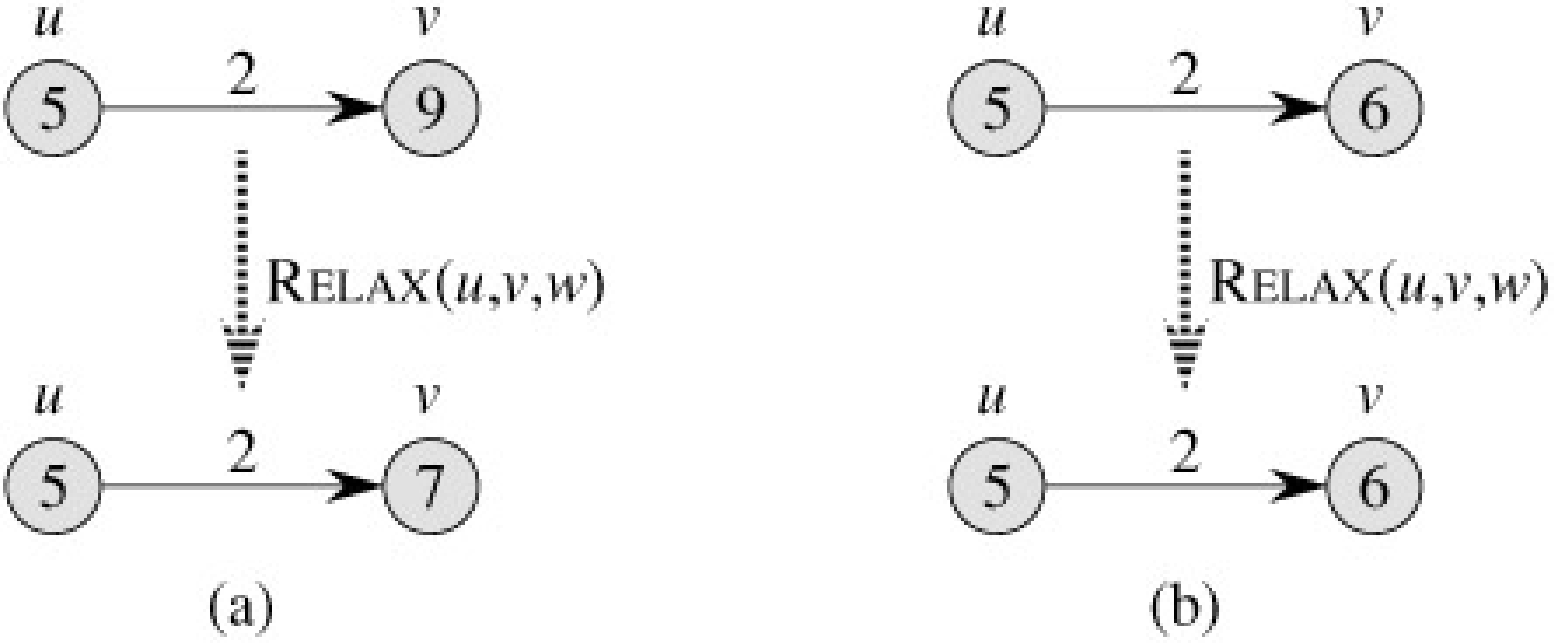
\includegraphics[width=\textwidth]{27.1}
				\label{fig:27.1}
			\end{figure}
		\end{minipage}
		\\\bottomrule
	\end{tabular}
\end{table}

\textbf{The algorithms differ in the order and how many times they relax each edge.}
\begin{answer}
	\begin{figure}[H]
		\centering
		\begin{tikzpicture}
			\begin{scope}\globalnodeset
				\node[label=left:Source] (S) at (0,0) {$0$};
				\node[label=above:A] (A) at (2,4) {$\infty$};
				\node[label=above:B] (B) at (8,0) {$\infty$};
				\node[label=below:C] (C) at (2,-4) {$\infty$};
				\node[label=below:D] (D) at (6,-4) {$\infty$};
			\end{scope}
			\begin{scope}\globalpathset
				\path [->] (A) edge node {$7$} (B);
				\path [->] (B) edge node {$2$} (D);
				\path [->] (D) edge node {$2$} (A);

				\path [->] (D) edge node {$5$} (C);
				\path [->] (C) edge node {$3$} (D);

				\path [->] (S) edge node {$3$} (A);

				\path [->] (S) edge[bend left=10] node {$-3$} (C);
				\path [->] (C) edge[bend left=10] node {$4$} (S);
			\end{scope}
		\end{tikzpicture}
		\label{fig:27.example}
	\end{figure}
\end{answer}

\section{Shortest Path Algorithm - Bellman-Ford}\label{sec:shortest-path-algorithm-bellman-ford}
The most straightforward of the ``relax an edge'' algorithms.%
\footnote{\begin{answer}Works on any graph with no negative cycles, and the algorithm finds the negative cycles.\end{answer}}
Relaxes the edges in a fixed order (any fixed order) $|V|-1$ times.%
\footnote{Most \# of edges on short path.}
Not a greedy algorithm.
\begin{itemize}
	\item Allows negative-weight edges.
	\item Computes $d[v]$ and $\pi[v]$ for all $v\in V$.
	\item Returns TRUE if no negative-weight cycles are reachable from $s$, FALSE otherwise.
\end{itemize}

\begin{table}
    \centering
	\label{tab:bellman-form}
	\begin{tabular}{|c|c|}
		\toprule
		\begin{minipage}[t]{0.6\textwidth}
			\begin{algorithm}[H]
				\caption{Bellman-Form Shortest Path Algorithm \begin{answer}$O(|V||E|)=O(|V|^{3})$\end{answer}}\label{alg:bellman-ford}
				\begin{algorithmic}[1]
				\Function{Bellman-Ford}{$V$, $E$, $w$, $s$}
					\State \Call{\hyperref[alg:init-single-source]{Init-Single-Source}}{$V$, $s$}
					\For{$i\gets1$ to $|V|-1$}%
						\ForAll{edge $(u,v)\in E$}
							\State \Call{\hyperref[alg:relax]{Relax}}{$u$, $v$, $w$}
						\EndFor
					\EndFor
					\ForAll{edge $(u,v)\in E$}\State\Comment{All edges, in any order, same order each time}
						\If{$d[v] > d[u] + w(u,v)$}%
							\begin{answer}\Comment{Must be a negative cycle}\end{answer}
							\State \Return FALSE
						\EndIf
					\EndFor
					\State \Return TRUE
				\EndFunction
				\end{algorithmic}
			\end{algorithm}
		\end{minipage} & \begin{minipage}[t]{0.43\textwidth}
			\begin{figure}[H]
				\centering
				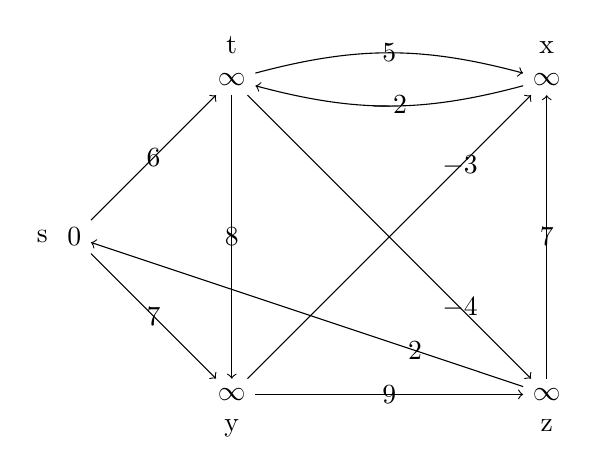
\begin{tikzpicture}
					\begin{scope}\globalnodeset
						\node[label=above:t] (t) at (0,0) {$\infty$};
						\node[label=above:x] (x) at (4,0) {$\infty$};
						\node[label=below:y] (y) at (0,-4) {$\infty$};
						\node[label=below:z] (z) at (4,-4) {$\infty$};
						\node[label=left:s] (s) at (-2,-2) {$0$};
					\end{scope}
					\begin{scope}\globalpathset
						\path [->] (t) edge[bend left=15] node {$5$} (x);
						\path [->] (x) edge[bend left=15] node {$-2$} (t);

						\path [->] (t) edge[near end] node {$-4$} (z);
						\path [->] (y) edge[near end] node {$-3$} (x);

						\path [->] (z) edge node {$7$} (x);
						\path [->] (t) edge node {$8$} (y);
						\path [->] (y) edge node {$9$} (z);

						\path [->] (z) edge[near start] node {$2$} (s);
						\path [->] (s) edge node {$7$} (y);
						\path [->] (s) edge node {$6$} (t);
					\end{scope}
				\end{tikzpicture}
				\label{fig:27.2}
			\end{figure}
		\end{minipage}
		\\\bottomrule
	\end{tabular}
\end{table}

\begin{enumerate}[start=3]
    \item Execute \Call{Bellman-Ford}{} on the above graph from source $s$ for this edge order
	$(t,x), (t,y), (t,z), \\(x,t), (y,x), (y,z), (z,x), (z,s), (s,t), (s,y)$.
	Update the $d[v]$ and $\pi[v]$ values for each iteration.
\end{enumerate}

\begin{answer}
	\begin{figure}[H]
		\centering
		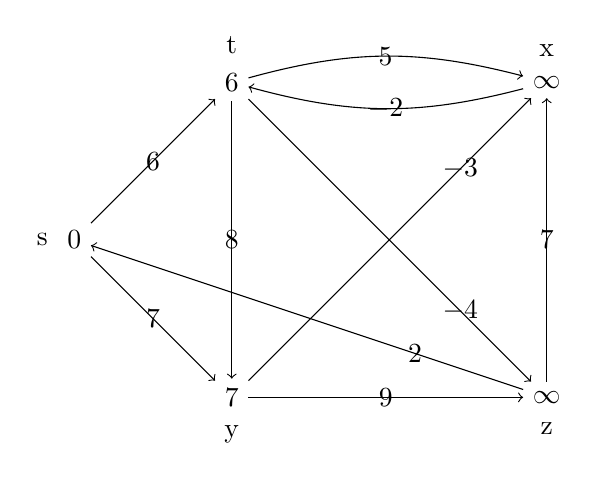
\begin{tikzpicture}
			\begin{scope}\globalnodeset
				\node[label=above:t] (t) at (0,0) {$6$};
				\node[label=above:x] (x) at (4,0) {$\infty$};
				\node[label=below:y] (y) at (0,-4) {$7$};
				\node[label=below:z] (z) at (4,-4) {$\infty$};
				\node[label=left:s] (s) at (-2,-2) {$0$};
			\end{scope}
			\begin{scope}\globalpathset
				\path [->] (t) edge[bend left=15] node {$5$} (x);
				\path [->] (x) edge[bend left=15] node {$-2$} (t);

				\path [->] (t) edge[near end] node {$-4$} (z);
				\path [->] (y) edge[near end] node {$-3$} (x);

				\path [->] (z) edge node {$7$} (x);
				\path [->] (t) edge node {$8$} (y);
				\path [->] (y) edge node {$9$} (z);

				\path [->] (z) edge[near start] node {$2$} (s);
				\path [->] (s) edge node {$7$} (y);
				\path [->] (s) edge node {$6$} (t);
			\end{scope}
		\end{tikzpicture}
		\caption{Example of the Execution of Bellman-Ford Step 1.}
		\label{fig:bellman-ford-example-1}
	\end{figure}
\end{answer}

\begin{enumerate}[start=4]
	\item What is the runtime of Bellman-Ford?
	\begin{answer}
		$O(|V||E|)=O(|V|^{3})$
	\end{answer}
	\item Prove Bellman-Ford is correct.\\
	Values you get on each pass how quickly it converges depends on order of relaxation.
	But guaranteed to converged after $|V|-1$ passes, assume no negative-weight cycles.
\end{enumerate}

%</Lecture-Activity-27>

\end{document}